

%\subsection{Setup}

%\paragraph{Tested optimizers}
We implement KFAC, KFAC*, as well as the diagonal, block-diagonal, and
full-Gramian ENGD in PyTorch~\citep{paszke2019pytorch}.
As a matrix-free version of ENGD, we use the HessianFree optimizer~\citep{martens2010deep} which uses truncated CG with exact Gramian-vector products to pre-condition the gradient.
We chose this because there is a fully-featured implementation from~\citet{tatzel2022late} which offers many additional heuristics such as adaptive damping, CG backtracking, and backtracking line search, which allows this algorithm to be operated with very little hyperparameter searching.
As first order-optimizers, we consider SGD with a tuned learning rate and momentum, as well as Adam with a tuned learning rate.
%
%\paragraph{Experimental setup}
We tune all hyper-parameters including step-sizes, momentum, the exponential-moving-average\todo{tba} parameter using Weights \& Biases~\citep{wandb} via random search, where we will make the runs and choices available after acceptance.
All experiments are run on a compute cluster with RTX 6000 GPUs (24\,GiB RAM).


\paragraph{A pedagogical example: 2d Poisson equation}

We consider a low-dimensional Poisson equation used to demonstrate the efficacy of energy natural gradients by~\cite{muller2023achieving}
as we can use it as a baseline here for its KFAC approximation.
The %problems are given by the two-dimensional
Poisson equation is given by
\begin{align}\label{eq:2D-Poisson}
    \begin{split}
        -\Delta u(x,y) & = 2\pi^2 \sin(\pi x) \sin(\pi y) \quad \text{for } (x,y)\in[0,1]^2 \\
    u(x,y) & = 0 \quad \text{for } (x,y) \in\partial[0,1]^2.
    \end{split}
\end{align}
%as well as the one-dimensional heat equation

\begin{comment}
    \begin{align}\label{eq:1D-Heat}
    \begin{split}
        \partial_t u(t,x) &= \kappa\partial_x^2u(t,x) \quad \text{for }(t,x)\in[0,1]^2
        \\
        u(0,x) &= \sin(\pi x) \qquad\;\, \text{for }x\in[0,1]
        \\
        u(t,x) &= 0 \qquad\qquad\quad\text{for }(t,x)\in[0,1]\times\{0,1\}.
    \end{split}
\end{align}
Here, we choose the heat-conductivity $\kappa = \frac14$ in our experiments.
\end{comment}

We evaluate the performance of the different optimizers for different network architectures with $4$ hidden layers of different widths and the hyperbolic tangent $\tanh$ as an activation function, where we allow the same computation time for all optimizers. 
Here, we only include the exact second-order methods when the parameter space of the network is small enough for this to be feasible.
As the equation admits a closed-form explicit solutions, we report the relative $L^2$ errors against the wall clock time achieved by the different optimizers in \Cref{fig:2D-Poisson}. 
%We are able to reproduce the results of~\cite{muller2023achieving} 
For networks of small size, we can reproduce the results of~\cite{muller2023achieving}, where exact ENGD achieves high accuracy, but in terms of computation time KFAC is competitive with the second-order optimizers. 
In contrast to ENGD which relies on an exact solution of the preconditioning step, KFAC scales to larger networks and is again competitive to other second-order optimizers that use much more sophisticated heuristics. 
\begin{figure}[t]
    \centering
    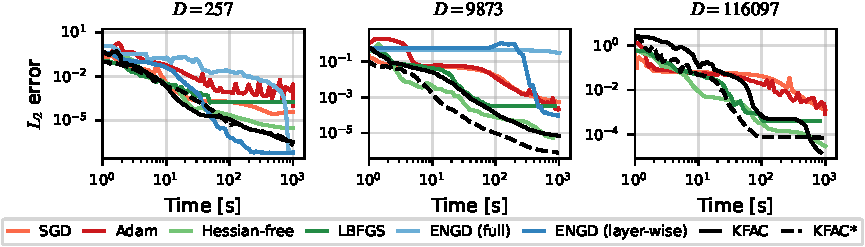
\includegraphics{../kfac_pinns_exp/exp17_groupplot_poisson2d/l2_error_over_time.pdf}
    \caption{We report the performance of different optimizers on the 2D Poisson equation~\eqref{eq:2D-Poisson} measured in relative $L^2$ error against wall clock time for architectures with different parameter dimensions $D$.}
    \label{fig:2D-Poisson}
\end{figure}
\begin{comment}
    \begin{figure}
    \centering
    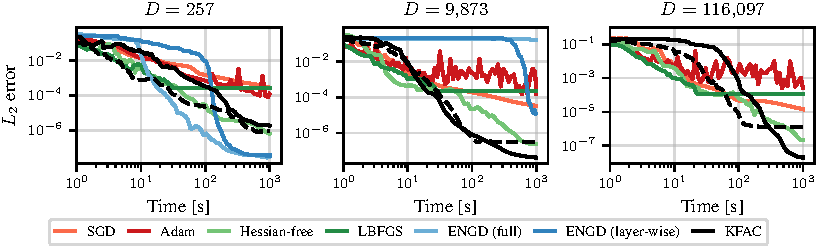
\includegraphics{kfac_pinns_exp/exp24_heat1d_groupplot/l2_error_over_time.pdf}
    \caption{We report the performance of different optimizers on the Poisson equation~\eqref{eq:2D-Poisson} measured in relative $L^2$ error against wall clock time for architectures with different parameter dimensions $D$; ...}
    \label{fig:2D-Poisson}
\end{figure}
\end{comment}

\paragraph{An evolutionary problem: (4+1)d heat equation}

To demonstrate that our method can also be applied to other problems as the Poisson equation we consider the four-dimensional heat equation
\begin{align}\label{eq:4D-heat}
     \partial_t u(t,x)-\kappa\Delta_x u(t,x) & = 0 \quad \text{for } t\in[0,1], x\in [0,1]^{4} \\
    u(0,x) & = \sum_{i=1}^{4} \sin(2 x_i) \quad \text{for }
     x\in [0,1]^{4}
     \\
     u(t,x) & = \exp(-t) \sum_{i=1}^{4} \sin(2 x_i) \quad \text{for } t\in[0,1], x\in\partial[0,1]^{4}
\end{align}
with $\kappa = 1/4$. Like before, we evaluate the performance of the different optimizers for networks with $4$ hidden layers, $\tanh$ activation function, and layers of different sizes.
We report the relative $L^2$ error with respect to the optimization time in \Cref{fig:4D-heat}.
Due to the higher spatial dimension, we use mini-batches in the evaluation of the loss and the preconditioner, where for KFAC, we keep the same batch for $100$ iterations.\todo{for the other optimizers?} 
Again, we observe that KFAC offers competitive performance compared with other second-order order optimizers that use sophisticated heuristics. 
\begin{figure}
    \centering
    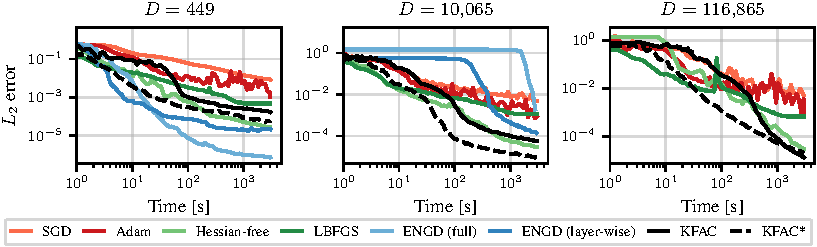
\includegraphics{../kfac_pinns_exp/exp30_heat4d_groupplot/l2_error_over_time.pdf}
    \caption{We report the performance of different optimizers on the 4D heat equation~\eqref{eq:4D-heat} measured in relative $L^2$ error against wall clock time for architectures with different parameter dimensions $D$.}
    \label{fig:4D-heat}
\end{figure}


\paragraph{High-dimensional Poisson equations}
We consider Poisson equations in dimensions $d=5,10,100$ on the problems used by~\cite{yu2018deep, muller2023achieving}, which admit the solutions 
\begin{align}\label{eq:solutions_poisson}
    \begin{split}
        u^\star(x) & = \sum_{i=1}^5 \cos(\pi x_i)? \quad \text{for } x\in [0,1]^{5}, \\
        u^\star(x) & = \sum_{k=1}^5 x_{2k-1}x_{2k},  \quad \text{for } x\in [0,1]^{10} \\ 
        u^\star(x) & = \lVert x \rVert_2^2 \quad \text{for } x\in [0,1]^{100}, 
    \end{split}
\end{align}
respectively. 
\begin{comment}
    \begin{align}\label{eq:5d_poisson}
    \begin{split}
        -\Delta u(x) & = -\sum_{i=1}^5 \cos(\pi x_i)? \quad \text{for } x\in [0,1]^{5} \\
    u(x) & = 0 \quad \text{for } x\in \partial[0,1]^{5}
    \end{split}
\end{align}
\begin{align}\label{eq:10d_poisson}
    \begin{split}
        -\Delta u(x) & = 0 \quad \text{for } x\in [0,1]^{10} \\
    u(x) & = \sum_{k=1}^5 x_{2k-1}x_{2k} \quad \text{for } x\in \partial[0,1]^{10}
    \end{split}
\end{align}
\begin{align}\label{eq:high_dimensional_poisson}
    \begin{split}
        -\Delta u(x) & = -2d \quad \text{for } x\in [0,1]^{100} \\
    u(x) & = \lVert x \rVert_2^2 \quad \text{for } x\in \partial[0,1]^{100}. 
    \end{split}
\end{align}
\end{comment}
%We test the different optimizers on problems with different spatial dimensions $d=5, 10, 100$ and 
Here, we select the hyper-parameters via a Bayesian optimization procedure. 
Again, we use mini-batches for $100$ iterations before drawing news samples. 
\todo{add verdict}


\begin{figure}
    \centering
    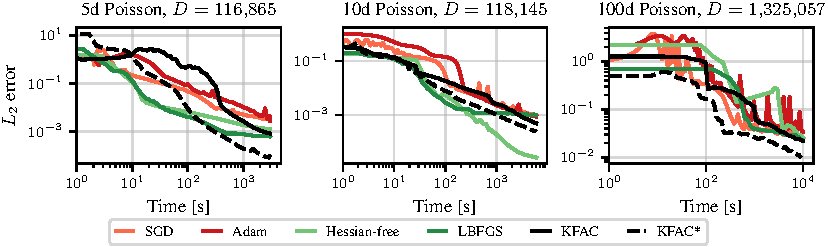
\includegraphics{../kfac_pinns_exp/exp33_poisson_bayes_groupplot/l2_error_over_time.pdf}
    \caption{
    We report the performance of different optimizers on Poisson equations in different spatial dimensions measured in relative $L^2$ error against wall clock time for a network with $D$ parameters; Bayesian optimization is used for the choice of the hyper-parameters.
    }
    \label{fig:10D-Poisson}
\end{figure}

%\todo[inline]{I think we should only present the time plots to safe space, move everything else to the appendix}

\begin{comment}
    \subsection{A 100D Poisson equation}

\begin{itemize}
\item 100D from deep Ritz paper~\citep{yu2018deep}, i.e.,
  \begin{align*}
    -\Delta u(x) & = -200 \quad \text{for } x\in [0,1]^{100} \\
    u(x) & = \lVert x \rVert_2^2 \quad \text{for } x\in \partial[0,1]^{100}
  \end{align*}
  where the solution is given by $u^\star(x) = \lVert x \rVert_2^2$
\item around $10^5$ to $10^6$ parameters
\item no ENGD, ENGD matrix-free?, only KFACs, L-BFGS, HF, and first-order methods
\end{itemize}


    \subsection{Heat equation}

\begin{itemize}
\item again 100D
\item sum of cosinuts with exponential trash in time? I.e.,
  time-space domain $[0,1]\times[0,1]^{100}$ %and
  % \begin{align*}
  %   \partial_t u(t,x)-\Delta_x u(t,x) & = 0 \quad \text{for } x\in [0,1]^{100} \\
      %       u(0,x) & = \sum_{i=1}^{100} \sin(\pi x_i) \quad \text{for }
  %   x\in [0,1]^{100}
  %   \\
  %   u(t,x) & = 0 \quad \text{for } t\in[0,1], x\in\partial[0,1]^{100}
  % \end{align*}
  % \item an alternative would be
  \todo{rhs not equal zero I think, double check before implementing}
  \begin{align*}
    \partial_t u(t,x)-\Delta_x u(t,x) & = 0 \quad \text{for } x\in [0,1]^{100} \\
    u(0,x) & = \sum_{i=1}^{100} \sin(\pi x_i) \quad \text{for }
             x\in [0,1]^{100}
    \\
    u(t,x) & = e^{-\pi^2 t}\sum_{i=1}^{100} \sin(\pi x_i) \quad \text{for } t\in[0,1], x\in\partial[0,1]^{100}
  \end{align*}
  for which the solution should be given by
  \begin{align*}
    u^\star(t,x) = e^{-\pi^2 t} \sum_{i=1}^{100} \sin(\pi x_i)?
  \end{align*}
  % we can also scale in time because $e^{-4\pi^2}\approx e^{-40}$
\item around $10^5-10^6$ parameters
\end{itemize}
\end{comment}

%\subsection{Limitations and Future Work}

\begin{comment}
  We want to show the following things:
  \begin{itemize}
  \item We can safely discard the Gramian's off-diagonal blocks without harming
    training performance. This reduces the Gramian's size, but still imposes
    strong constraints on scalability.

  \item Our proposed Kronecker approximation works roughly as well as the
    full/block diagonal Gramian, while being much cheaper to compute, store, and
    invert.

  \item Thanks to the Kronecker approximation of the Gramian, we can scale to larger neural networks where the other methods either do not work (storing the Gramian is prohibitively expensive) or become quite slow (matrix-free linear system solve via Gramian-vector products).
  \end{itemize}

  Todos:
  \begin{itemize}
  \item concrete example ground truth: 2d Poisson on unit square with sine target
  \end{itemize}

  Ideas:
  \begin{itemize}
  \item try out different approximations
    \begin{itemize}
    \item Ground truth
    \item Block diagonal exact
    \item Diagonal
    \item Block diagonal with different approximations
    \end{itemize}
  \end{itemize}
\end{comment}

%%% Local Variables:
%%% mode: latex
%%% TeX-master: "../main"
%%% End:
